\documentclass{article}
\usepackage{amsmath,amsthm,mathrsfs,amssymb,graphicx,hyperref,url}
\usepackage{geometry}
\title{PHYS 215C In-Class Notes}
\author{Bill Wolf, Keith Fratus}
\date{Spring 2011}
\begin{document}
\maketitle \newpage{}
\tableofcontents
 \newpage{}
		\textit{March 28, 2011}	
	\section{Scattering}
		\subsection{Suggested References}
		\begin{itemize}
			\item Sakurai Ch. 6
			\item Shankar Ch. 19
			\item Merzbacher Ch. 11
		\end{itemize}
		\subsection{Basic Setup}
		The basic idea in scattering theory is a particle being scattered into a target (particle into target). Other models model two particles moving towards each other and scattering off each other (particle into particle).
		\subsubsection{Applications}
		Particle into particle scattering is very prevalent in high energy physics studies (particle accelerators), with traditional subatomic particles like electrons, neutrons, and protons.\\
		
		\noindent Target scattering is used to model particle-particle interactions (particle physics), atoms and ions (atomic/nuclear physics), and interactions within a solid or liquid (condensed matter physics).
		
		\subsection{Scattering Approach to ${e^-}$ Transport in solids}
		\subsubsection{Setup}
		In this theory we talk about the conduction of electrons in a metal or doped semiconductor. The canonical experiment is a battery providing a potential difference across the material of interest. The conductance, $G=I/V=1/R$, is what is of interest. There are impurities in the metal or semiconductor that cause scattering of the electrons that are moving under the influence of the potential difference.
		\subsubsection{Rolf Landauer's Theory (Landauer Transport Theory)}
		\paragraph{Toy Model} Consider a one-dimensional scattering potential that is a finite potential barrier between $x=a$ and $x=-a$ with incident electrons coming from the left with average energy $E$. (This is actually very relevant in a gated two-dimensional electron gas, where the low energies only allow one mode on the surface dimension.) The theory of this problem is well understood in terms of transmission and reflection coefficients (see the appendix in Sakurai). We will look at the \emph{steady state} system.\\
		
		\noindent First divide the region up into three regions. Region I is $-\infty<x<-1$, region II is $-a<x<a$, and region III is $a<x<\infty$. This gives rise to three wave functions of interest.
		\begin{align*}
			\psi_{\mathrm{I}}&=A_{\mathrm{in}}e^{ikx}+A_{\mathrm{out}}e^{-ikx}\\
			\psi_{\mathrm{II}}&=C_1e^{ik'x}+C_2e^{-ik'x}\\
			\psi_{\mathrm{III}}&=B_{\mathrm{out}}e^{9kx}+B_{\mathrm{in}}e^{-ikx}
		\end{align*}
		where $$k=\frac{1}{\hbar}\sqrt{2mE}\qquad k'=\frac{1}{\hbar}\sqrt{2m(E-V)}$$
Normally we would solve for these wave functions by matching $\psi$ and $\psi'$ at the boundaries to relate $A,B,$ and $C$. We can represent the solution via a transfer matrix:
$$\left(\begin{array}{c}B_{\mathrm{out}} \\B_{\mathrm{in}}\end{array}\right)=\left(\begin{array}{cc}M_{11} & M_{12} \\M_{21} & M_{22}\end{array}\right)\left(\begin{array}{c}A_{\mathrm{in}} \\A_{\mathrm{out}}\end{array}\right)$$


% I need to get the figure file from Bill - Keith
% Done! 4/2/2011 - Bill
\begin{figure}[h]
	\centering
	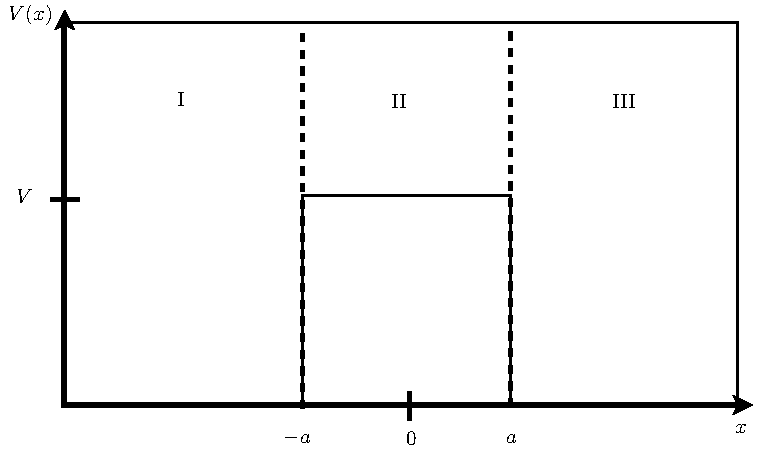
\includegraphics{Fig_1}
	\caption{1-D Scattering Potential}
\end{figure}
Alternatively, we may use the less clear $S$-matrix:
			$$\left(\begin{array}{c}A_{\mathrm{out}} \\B_{\mathrm{out}}\end{array}\right)=\left(\begin{array}{cc}S_{11} & S_{12} \\S_{21} & S_{22}\end{array}\right)\left(\begin{array}{c}A_{\mathrm{in}} \\B_{\mathrm{in}}\end{array}\right)$$
			The system obeys an equation of continuity (probability conservation):
			$$\partial_t\left|\psi\right|^2+\partial_xJ=0$$
			where
			$$J=\frac{\hbar}{m}\mathrm{Im}\left(\psi^*\partial_x\psi\right)$$
			The currents in regions I and III gives
			\begin{align*}
				J_{\mathrm{I}}&=\frac{\hbar k}{m}\left[\left|A_{\mathrm{in}}\right|^2-\left|A_{\mathrm{out}}\right|^2\right]\\
				J_{\mathrm{III}}&=\frac{\hbar k}{m}\left[\left|B_{\mathrm{out}}\right|^2-\left|B_{\mathrm{in}}\right|^2\right]
			\end{align*}
			The equation of continuity then tells us that
			$$\left|A_{\mathrm{out}}\right|^2+\left|B_{\mathrm{out}}\right|^2=\left|A_{\mathrm{in}}\right|^2+\left|B_{\mathrm{in}}\right|^2$$
			$$\left(\begin{array}{cc}A_{\mathrm{out}}^* & B_{\mathrm{out}}^*\end{array}\right)\left(\begin{array}{c}A_{\mathrm{out}} \\A_{\mathrm{out}}\end{array}\right)=\left(\begin{array}{cc}A_{\mathrm{in}}^* & B_{\mathrm{in}}^*\end{array}\right)S^\dagger S\left(\begin{array}{c}A_{\mathrm{in}} \\B_{\mathrm{in}}\end{array}\right)$$
			For scattering states, we let $B_{\mathrm{in}}=0$, that is, particles are \emph{only} incident from the left. Then we have
			$$\psi_k(x)=\begin{cases} A_{\mathrm{in}}e^{ikx}+A_{\mathrm{out}}e^{-ikx} & x<-a\\
			B_{\mathrm{out}}e^{ikx} &x>a \end{cases}$$
			and we have
			\begin{align*}
				B_{\mathrm{out}}&=S_{21}A_{\mathrm{in}}\\
				A_{\mathrm{out}}&=S_{11}A_{\mathrm{in}}
			\end{align*}
			We define transmission and reflection coefficients
			\begin{align*}
			T&\equiv \frac{\left|B_{\mathrm{out}}\right|^2}{\left|A_{\mathrm{in}}\right|^2}=\left|S_{21}\right|^2\\
			R&\equiv \frac{\left|A_{\mathrm{out}}\right|^2}{\left|A_{\mathrm{in}}\right|^2}=\left|S_{11}\right|^2\\
			\end{align*}
			\paragraph{Landauer Formula}
			$$G=\frac{I}{V}\Rightarrow G=\frac{e^2}{h}T$$
			where $e^2/h$ is the quantum of conductance.\\
			
			\noindent \textit{March 30, 2011}
			\subsubsection*{Derivation of the Landauer Formula}
			Suppose we send in a wave with wave number $k$ and energy $E=\hbar^2k^2/2m$ from the left. As expected, we would get a portion of the wave to be reflected (proportional to $S_{11}$) the remainder to to be transmitted (proportional to $S_{21}$).	\\		
			
			\noindent The Scattering State is then given by
			$$\psi_{1}^k(x)=\begin{cases} \frac{e^{i\phi_1 k}}{\sqrt{2\pi}}\left(e^{ikx}+S_{11}e^{-ikx}\right) & x<-a\\
			\frac{e^{\phi_1k}}{\sqrt{2\pi}}S_{21}e^{ikx} & x>a \end{cases}$$
			$$\psi_2^k(x)=\begin{cases} \frac{e^{i\phi_2 k}}{\sqrt{2\pi}}\left(e^{ikx}+S_{22}e^{ikx}\right) & x>a\\
			\frac{e^{\phi_2k}}{\sqrt{2\pi}}S_{12}e^{-ikx} & x<-a \end{cases}$$
			With this, we are ready to\ldots\\
			
			\noindent For $T=0$, we have incident electrons up to chemical potential $\mu$. On different leads on a quantum wire, we generally have two different chemical potentials, which causes a net transport of electrons. Suppose on the left we have $\mu_1$ and on the right we have $\mu_2$ with $\mu_1<\mu_2$, which causes an electrical net current from left to right. Our goal is to study this current in terms of the $S$-matrix.
			\paragraph{Fermi Wave Number} We define the Fermi Wave Number by
			$$k_F=\frac{1}{\hbar}\sqrt{2m\mu}$$
			The probability current for $e^{-1}$ at $k$ is given by
			$$J_j^k=\frac{\hbar}{m}\mathrm{Im}\left[{\psi_j^k}^*(x)\partial_x \psi_j^k(x)\right]$$
			The electrical current is then
			$$\left.I\right|_{x>a}=e J_j^k=e\frac{\hbar}{m}\left[\int_0^{k_{F_1}}dk\,\frac{k}{2\pi}\left|S_{21}\right|^2+\int_{0}^{k_{F_2}}dk\frac{k}{2\pi}\left(-1+\left|S_{22}\right|^2\right)\right]$$
			Then the transmission probability if $T_k\equiv\left|S_{21}\right|^2$, which gives the current to be
			$$I=\frac{e}{2\pi}\int_{k_{F_2}}^{k_{F_1}}dk\,\left(\frac{\hbar k}{m}\right)T_k=\frac{3}{2\pi\hbar}\int_{\mu_2}^{\mu_1} dE\,T(E)$$
			Where we have used $E=\hbar2k^2/2m$ and $dE=(\hbar^2k/m)\,dk$. We may relate the two chemical potentials to the electric voltage via
			$$\mu_1=\mu_2+eV$$
			\paragraph{Linear Response}
			The conductance is given by 
			$$G=\lim_{V\to0} \frac{I}{V}$$
			Then the electric current can be rewritten as
			$$I=\frac{e}{2\pi\hbar}\int_{\mu_2}^{\mu_2+eV}dE\,T(e)=\frac{e^2}{h}T(\mu)V$$
			and then the conductance in this linear response limit is
			$$G=\frac{I}{V}=\frac{e^2}{h}T(\mu)=\frac{e^2}{h}T(E_F)$$
			\subsubsection{Some Comments}
			\begin{enumerate}
				\item Suppose we have a perfect wire with \emph{no} backscattering. That is, $T=1$. Then we have $R=\frac{1}{G}=0$. This would of course be superconductivity.
				\item This theory can be generalized to multichannel wires with many leads. The resulting conductance for $N$ leads is then
				$$G=\frac{e^2}{h}2N$$
				where the factor of 2 comes from electron spin degeneracy.
				\item This theory has been validated by experiment with a quantum wire circuit setup that revealed a stair-step plot of conductance as a function of input voltage.
				\item We have ignored the fact that the electrons interact and experience interactions off of one another (calculations effectively carried out at zero temperature). As a result, these resistances do not necessarily add in series.
			\end{enumerate}
			\subsection{Inelastic Scattering}
			In the field of inelastic scattering, we typically consider the situation of a particle scattering off of a quantum mechanical system. This system could be a liquid, a solid, a nuclei\ldots anything, really. The inelastic condition implies that the act of scattering transfers energy between the particle and the target. 
			
			\subsubsection{Setup and Notation} To ease the theory, we will suppose that the ``target'' will be composed of particles with position operators $\mathbf{R}_i$ and momentum operators $\mathbf{P}_i$. The incident particle will have position operator $\mathbf{R}$ and $\mathbf{P}$. The Hamiltonian of the system will be
			
			%%%%%%%%%
			$$\hat{\mathscr{H}}=\frac{\mathbf{P}^2}{2m}+\hat{H}+V$$
			%%%%%%%%%
			
			Where the first term is the kinetic energy of the particle, the non-script Hamiltonian is the internal energy of the target, and the potential is the interaction potential. To simplify the system, we shall assume that the interaction potential takes on the form
			
			
			$$V=\sum_{i=1}^N V(\mathbf{R}-\mathbf{R}_i)$$
			
			
			\paragraph{Density Operator} It becomes useful to define a density operator for the target. It is
			$$\rho(\mathbf{r})=\sum_{i=1}^N \delta^3(\mathbf{r}-\mathbf{R}_i)$$
			where $\mathbf{r}$ is simply a c-number position coordinate. We will use the Fourier transform of this operator,
			$$\rho(\mathbf{q})=\int d^3\mathbf{r}\,e^{-i\mathbf{q}\cdot\mathbf{r}}\rho(\mathbf{r})=\sum_{i=1}^Ne^{-i\mathbf{q}\cdot\mathbf{R}_i}$$
			\paragraph{Rewriting the Interaction Potential} This density operator can help us rewrite the potential into a more useful form:
			$$V=\sum_{i=1}^N \int\frac{d^3\mathbf{q}}{(2\pi)^3}V(\mathbf{q})e^{i\mathbf{q}\cdot(\mathbf{R}-\mathbf{R}_i}=\int\frac{d^3\mathbf{q}}{(2\pi)^3}V(\mathbf{q}) \rho(\mathbf{q})e^{i\mathbf{q}\cdot\mathbf{R}}$$
			\subsubsection{Modeling Scattering}
			\paragraph{Fermi's Golden Rule} Suppose we start with an initial state $\left|\mathbf{k};\,E_i,\alpha\right>$ where the $\alpha$ labels all states in target with the energy $E$ (may be degeneracy), and we end with a final state $\left|\mathbf{k}';\,E_f,\beta\right>$. Recall that Fermi's Golden Rule tells us
			$$\Gamma_{i\to f}=\frac{2\pi}{\hbar}\left|\left<\mathbf{k}';\,E_f,\beta\right|V\left|\mathbf{k};\,E_i,\alpha\right>\right|^2\delta(E_f+\epsilon_{k'}-E_i-\epsilon_k)$$
			The meaning of the delta function is clear. For brevity, we'll denote the matrix element as $V_{fi}$. In terms of the interaction potential, this matrix element is then
			$$V_{fi}=\int\frac{d^3\mathbf{q}}{(2\pi)^3}V(\mathbf{q})\left<\mathbf{k}';\,E_f\beta\left|\rho(\mathbf{q})e^{i\mathbf{q}\cdot \mathbf{R}}\right|\mathbf{k};\,E_i\alpha\right>$$
			We now make use of the fact that the momentum and position operators are conjugate operators:
			$$e^{ia\hat{p}/\hbar}\left|x\right>=\left|x+a\right>$$
			$$e^{iq\hat{x}}\left|k\right>=\left|k+q\right>$$
			So now we have
			$$e^{i\mathbf{q}\cdot\mathbf{R}}\left|\mathbf{k}\right>=\left|\mathbf{k}+\mathbf{q}\right>$$
			and
			$$\left<\mathbf{k}'\left| e^{i\mathbf{q}\cdot\mathbf{R}}\right|\mathbf{k}\right>=\left<\mathbf{k}'\right|\left.\mathbf{k}+\mathbf{q}\right>=\delta^3(\mathbf{k}'-\mathbf{k}-\mathbf{q})$$
			Then the matrix element is 
			$$V_{fi}=\frac{V(\mathbf{k}'-\mathbf{k})}{(2\pi)^3}\left<E_f\, \beta\left|\rho(\mathbf{k}'-\mathbf{k})\right|E_i\,\alpha\right>$$
			Now we are interested in calculating the differential cross-section, which is
			$$\left(\frac{d^2\sigma}{d\epsilon\,d\Omega}\right)d\Omega\, d\epsilon\equiv \frac{\textrm{\# of scattered particles/time into solid angle }d\Omega\textrm{ and energy }\epsilon\to\epsilon+d\epsilon}{\textrm{\# of incident particles/time-area}}$$
			Then using Fermi's Golden Rule,
			$$\Gamma_{i\to d\Omega\,d\epsilon}=\Gamma_{i\to f}{k'}^2dk'\,d\Omega=\Gamma_{i\to f}\left(\frac{m}{\hbar^2}\right)k'\,d\epsilon\,d\Omega$$
			With 
			$$\epsilon=\frac{\hbar^2{k'}^2}{2m}\Rightarrow d\epsilon=\frac{\hbar^2}{m}k'\,dk'$$
			The differential cross section is now
			$$\frac{d^2\sigma}{d\Omega\,d\epsilon}=\frac{\sum_{E_f, \beta}\left(\frac{m}{\hbar^2}\right)k'\Gamma_{i\to f}}{\left(\frac{1}{2\pi}\right)^3\left(\frac{\hbar k}{m}\right)}=\left(\frac{m}{2\pi \hbar^2}\right)^2\left|V(\mathbf{k}'-\mathbf{k})\right|^2\frac{k'}{k}\sum_{E_f,\beta}\delta(E_f+\epsilon_{k'}-E_i-\epsilon_k)\left|\left<E_f\,\beta\left|\rho(\mathbf{k}'-\mathbf{k})\right|E_i\,\alpha\right>\right|^2$$
			\paragraph{Dynamical Structure Factor} To simplify the form of the cross-section, we introduce the dynamical structure factor, defined as
			$$S(\mathbf{q},\omega)=\sum_{E_f\,\beta}\delta\left(\omega+\frac{E_f-E_i}{\hbar}\right)\left|\left<E_f\beta\left|\rho(\mathbf{q})\right|E_i\,\alpha\right>\right|^2$$
			where the inner product is a property only of the \emph{target}. Also, recall that $\mathbf{q}$ is the momentum transfer during scattering and $\omega$ is just the energy transfer divided by $\hbar$. Rewriting the delta function,
			$$S(\mathbf{q},\omega)=\sum_{E_f\,\beta}\int dt\,e^{i\omega t}e^{i(E_f-E_i)t/\hbar}\left<E_i\,\alpha\left|\rho(-\mathbf{q})\right|E_f\,\beta\right>\left<E_{f}\,\beta\left|\rho(\mathbf{q})\right|E_i\,\alpha\right>$$
			which can be further simplified by
			$$e^{it(E_f-E_i)/\hbar}\left<E_{f}\,\beta\left|\rho(\mathbf{q})\right|E_i\,\alpha\right>=\left<E_{f}\,\beta\left|e^{i Ht/\hbar}\rho(\mathbf{q})e^{-iHt/\hbar}\right|E_i\,\alpha\right>$$
			So the dynamical structure factor is then
			$$S(\mathbf{q},\omega)=\int \frac{dt}{2\pi}e^{i\omega t}\left<E_I\,\alpha\left|\rho(-\mathbf{q},0)\rho(\mathbf{q},t)\right|E_i\,\alpha\right>$$
			Supposing the target is at some temperature $T$, for some operator $\hat{\theta}$,
			$$\left<\hat{\theta}\right>\equiv \frac{1}{Z}\sum_{E,\alpha}e^{-\beta E}\left<E_\alpha\left|\hat{\theta}\right|E\,\alpha\right>;\qquad Z=\sum_{E\,\alpha}e^{-\beta E}$$
			\begin{center}
				\fbox{$\displaystyle S(\mathbf{q},\omega)=\int\frac{dt}{2\pi}e^{i\omega t}\left<\rho(-\mathbf{q},0)\rho(\mathbf{q},t)\right>$}
			\end{center}
			\paragraph{Some Comments}
			\begin{enumerate}
				\item If we don't measure the final energy (i.e. we measure the \emph{direction}),
				$$S_{\mathrm{static}}(\mathbf{q})=\int d\omega S(\mathbf{q},\omega)=\left<\rho(-\mathbf{q})\rho(\mathbf{q})\right>=\left<\left|\sum_ie^{-\mathbf{q}\cdot\mathbf{R}_i}\right|^2\right>$$
				\item If the target particles are very heavy (i.e. they do not move),
				$$\rho(\mathbf{q},t)=\rho(\mathbf{q})$$
				and
				$$S(\mathbf{q},\omega)=S(\omega)S_{\mathrm{static}}(\mathbf{q})$$
				\item (MISSING IMPORTANT FIGURE)\\
				
				\noindent For particles traveling with a path length differene, a phase difference is accumulated:
				$$\Delta \phi_i=\frac{2\pi}{\lambda}\hat{R}_i\hat{k}-\frac{2\pi}{\lambda'}\hat{R}_i\hat{k}'=\mathbf{R}_i\cdot(\mathbf{k}-\mathbf{k}')=-\mathbf{R}_i\cdot\mathbf{q}$$
			\end{enumerate}
			$$\mathrm{Amp}\approx \sum_i e^{i\Delta\phi_i}\cong \sum_ie^{-i\mathbf{q}\cdot\mathbf{R}_i}=\rho(\mathbf{q})$$
			So the scattered intensity is
			$$S(\mathbf{q})\sim\left<\left|\mathrm{Amp}\right|\right>=\left<\rho(\mathbf{q})\rho(-\mathbf{q})\right>$$
			\subsubsection{Scattering Examples}
			Suppose we scatter off of a solid or liquid with length scale $a\sim$ 3\AA\  and energy scale $k_BT_{\mathrm{room}}\sim300\,\mathrm{K}$.
			\paragraph{Light Scattering} 
			$$\epsilon=\hbar\omega=\hbar ck=\frac{hc}{\lambda}\approx 10^4\,\mathrm{eV}\sim10^7\,\mathrm{K}$$
			$$\Delta \epsilon\sim 300\,\mathrm{K}$$
			This is in fact X-Ray scattering.
			
				
\end{document}